\section{September 9, 2021} 
Last time we talked about limits and colimits, some examples being products and coproducts, fiber products, equalizers and coequalizers, completion and localization. To describe finite limits and colimits in $\mathsf{Set} $, in some sense you only need to understand products and coproducts, equalizers and coequalizers.

Consider a diagram of sets, where $\{A_i \} _{i \in I}$ sets, $\{A_i  \xrightarrow{f_{ij}^k} \} $. The basic limit is the product of the $A_i $'s, $\prod A_i $. This is the limit of two (or $n$) dots without arrows between them. To justify the slogan ``limits are subs, colimits are quotients'', $\varprojlim \{A_i \} $ is a subset of $\prod A_i $. We have \[
    \varprojlim \{A_i \} = \{(\cdots , a_i , a_j , \cdots ) \in \prod A_i  \mid  f_{ij}^k (a_i )=a_j \ \text{for all} \ i,j,k\} .
\] An exercise is to check that this satisfies the universal property. For the colimit, the claim is that $\varinjlim A_i =\coprod A_i  / \sim$, the question is now ``what is this equivalence relation?'' The relation is described by $\sim \colon$ the minimal equivalence relation containing $a_j  \sim f_{ij}^k a_i $, $A_i \xrightarrow{f_{ij}^k} A_j $. 

We can think of \textbf{filtered diagrams} as ``trying to have'' a final object. Filtered diagrams have ``direction'': this means that for any two arrows $t_1,t_2$, they eventually compose to a common place. Filtered diagrams typically don't have a final object as this would make the category uninteresting.
\begin{definition}[]
    A diagram $I$ is \textbf{filtered} if for all $A,B \in I$, there exists a $C$ such that
\[
\begin{tikzcd}
A \arrow[rrd] &  &   \\
              &  & C \\
B \arrow[rru] &  &  
\end{tikzcd}
\] 
    and any two morphisms  \[
   \begin{tikzcd}
       A \arrow[r, "f_1", shift left] \arrow[r, "f_2"', shift right] \arrow[rr, bend left, shift left] \arrow[rr, bend right, shift right] & B \arrow[r, dashed] & C
\end{tikzcd} 
    \] have coequalizers. 
\end{definition}
The colimit is ``trying to be the root of the tree'', or $\varinjlim_I \{A_i \} _{i \in I}=\coprod A_i / a_i  \in A_i  \sim A_j  \in A_j $ if there exists morphisms identifying $a_1,a_2$. When we say ``morphisms identifying'', this precisely means there exists \[
\begin{tikzcd}
a_i\in A_i \arrow[rrd, "g_1"]   &  &     \\
                                &  & A_N \\
a_j \in A_j \arrow[rru, "g_2"'] &  &    
\end{tikzcd}
\] such that $g_1(a_i )=g_2(a_j )$.
In general, filtered colimits behave much nicer with functors than other colimits.

\subsection{Adjoints}
Recall the method of least squares from linear algebra, where we need to define an inner product to define projections, giving a best approximation of $v$ that lives in $w$ (for $v\in  V,w \in W, W \subseteq V$). This is characterized by saying $\langle \mathrm{proj}_W w, w \rangle $ for $w \in W$ is equal to $\langle v,w \rangle $. Denote the inclusion by $i \colon W \hookrightarrow V $, so $\langle \mathrm{proj}_W, v,w \rangle _W= \langle v, i(w) \rangle _V$.

We generalize this notion in linear algebra by an adjoint map. Consider a map of inner product spaces $f \colon W \to V$. Then $f^{\dag} \colon V \to W$ is ``the best inverse'' for $f$, where $f^{\dag}$ is characterized by \[
\langle f ^{\dag}v, w \rangle _W=\langle v, fw \rangle _V.
\] Here is a schematic way of looking at it. 
\begin{figure}[H]
\centering
 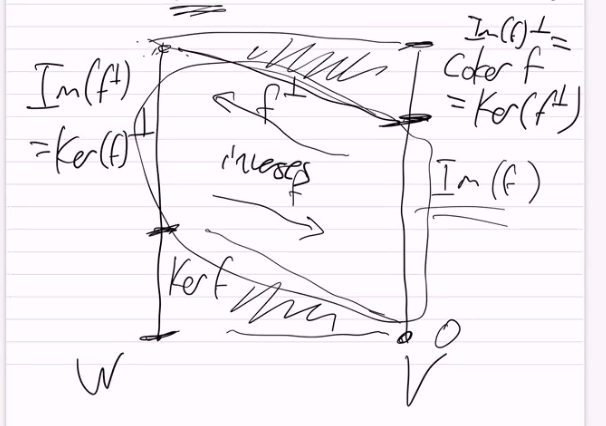
\includegraphics[width=0.6\linewidth]{figures/adjoint.png}
 \caption{Visualizing adjoints in linear algebra.} 
 \label{adj} 
\end{figure}
The kernel is collapsed to zero, and the cokernel is the remainder of the image. Then $\im f^{\dag}$ is the orthogonal complement of  $\ker f$ (which makes sense with an inner product), and $f$ and $f^{\dag}$ are inverses. This lifts the statement $\dim W-\dim \ker = \dim \im f$ to a statement about the spaces themselves.

Now we try to do the same thing in category theory. Instead of spaces, we have a functor between categories  $F \colon \mathcal{C}  \to \mathcal{D} $. The most crucial piece of data we are missing is the inner product. Given two objects $A,B \in \mathcal{C} $, we think of the pairing $\Hom _{\mathcal{C} }(A,B)$ as an inner product of sorts, a way of measuring the ``distance'' between the two. This is a non-symmetric inner product.

\begin{definition}[]
    Let $F \colon \mathcal{C}  \to \mathcal{D} $ be a functor. We say a functor $G \colon \mathcal{D}  \to \mathcal{C} $ is a \textbf{right adjoint} to $F$ if $\Hom _{\mathcal{C} }(A, G(B))\simeq \Hom _{\mathcal{D} }(F(A),B)$, where $A \in \mathcal{C} $, $B \in \mathcal{D} $ ``functorially in $A,B$''. We say $F$ is a \textbf{left adjoint} to $G$.\footnote{To remember this, note that $G$ is appearing on the right side of the $\Hom$'s and $F$ is appearing on the left side of the $\Hom$'s.}
\end{definition}
$\Hom _{\mathcal{C} }(-,G(-))\simeq  \Hom _{\mathcal{D} }(F(-),-)$ should be a natural isomorphism of functors $\mathcal{C} ^{\mathrm{op}}\times \mathcal{D} \to \mathsf{Set} $. To make sense of that last statement, let $\mathcal{C} $ be a category. Then $\Hom _{\mathcal{C} }(-,-) \colon \mathcal{C} ^{\mathrm{op}} \times \mathcal{C} \to \mathsf{Set} $ is a functor.

\begin{namedthing}{Notation} 
If $(F,G)$ are an adjoint pair, then $G$ is the right adjoint and $F$ is the left. We also use the notation $F\dashv G$ which comes from turning the perpendicular ($\perp$) sign sideways, since the relation is not symmetric.
\end{namedthing}
    
\begin{example}
    {\color{red}todo:free and forgetful functor} 
\end{example}
\begin{example}[Tensor products]
Suppose we have two vector spaces $V,W$ and we want to define $V \otimes W$. Then for a bilinear map $\varphi  \colon V \times W \to U$, the tensor product satisfies by a universal property \[
\begin{tikzcd}
                                           & V\otimes W \arrow[rd, "\exists!", dotted] &   \\
V\times W \arrow[ru] \arrow[rr, "\varphi"] &                                           & U
\end{tikzcd}
\]  or $\varphi (v,w) \in U, $ {\color{red}todo:STOP SCROLLING BY SO FAST} 
\end{example}
